\documentclass{article}
\usepackage{geometry,color,graphicx}
\usepackage{caption}
\usepackage{subcaption}
\usepackage{float}
\usepackage{amsmath}
\usepackage{empheq}

\graphicspath{ {../plots/} }

\begin{document}

\title{Project 3: Using the GNU Scientific Library and solving the Laplace equation }

\author{Gabriel Smadi\\
  Syracuse University,\\
  \texttt{gsmadi@syr.edu}}
\maketitle

\begin{abstract}
The GSL library is utilized to solve common computational problems such as root finding
and matrix computations. The Laplace equation is solved utilizing the method of over-relaxation.
The performance of some algorithms are explored and quantified, such as computing matrix determinants
and speedup improvements of solving the Laplace equation by using the optimal relaxation factor.
\end{abstract}

\section{Introduction}

Having the ability to implement numerical algorithms is useful yet can be error prone. The educational outcomes of implementing
such algorithms is fruitful, yet ill advised in production or formal research environments. The best practice when robust numerical
algorithms are needed is to utilized mature and thoroughly tested software libraries or packages. In this project, the GNU
Scientific Library (GSL) is utilized to solve some illustrative numerical problems and to get some experience using software
developed by others. Also, in this project we solve the Laplace equation b the method of over-relaxation. Solving the
Laplace equation numerically proves to be simple, yet by making use of a relaxation factor we will see how it greatly improves the
performance of the algorithm.

\section{Fraunhoffer Diffraction}

The Fraunhoffer diffraction amplitude is given by,

\begin{equation}
\label{eq:fraun_amp}
  A = A_{0}\frac{\sin{x}}{x}
\end{equation}

\begin{figure}[H]
  \begin{center}
    \scalebox{.6}{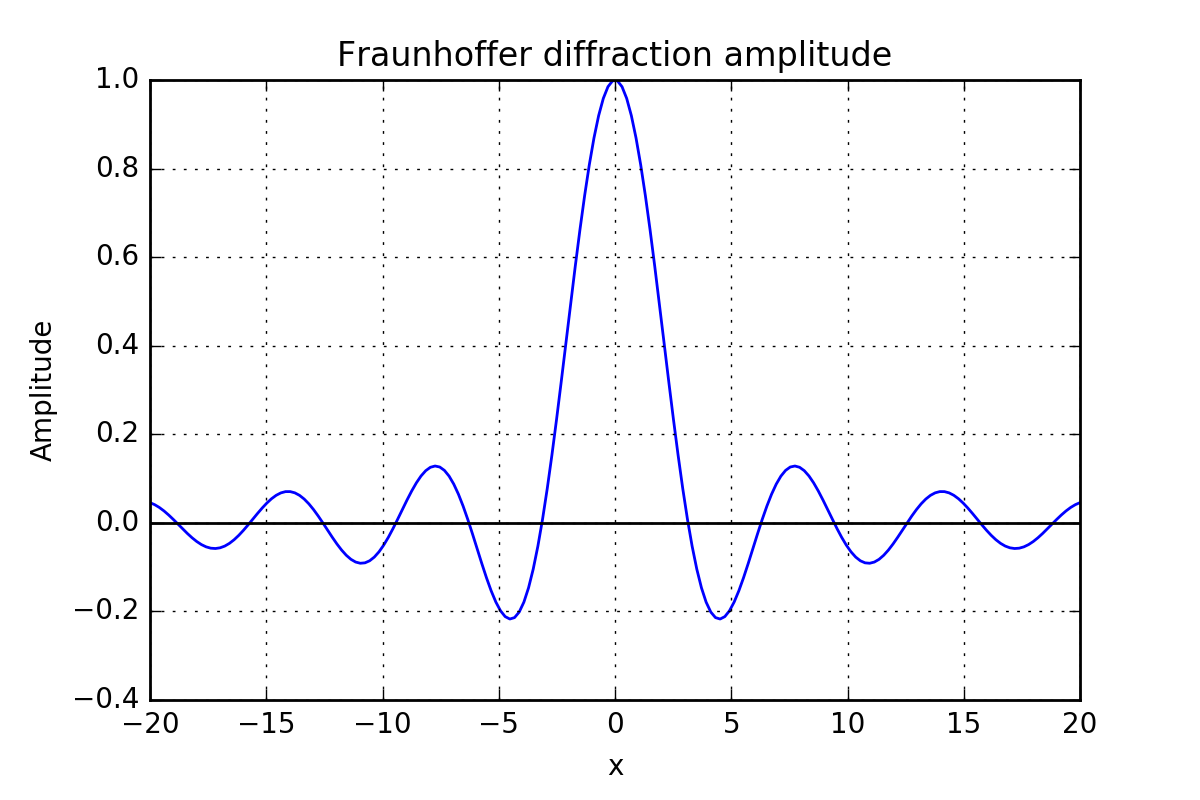
\includegraphics{fraun_amplitude}}
  \end{center}
  \caption{Fraunhoffer amplitude}
  \label{fig:fraun_amp}
\end{figure}

\begin{table}[H]
  \begin{center}
    \begin{tabular}{|c|c|c|c|}
      \hline
      Root & Angle(Radians) & Angle(Degrees) \\
      \hline
      4.493030 & 0.305737 & 17.52 \\
      \hline
      7.728195 & 0.544190 & 31.18 \\
      \hline
      10.906603 & 0.819277 & 46.94 \\
      \hline
      14.069672 & 1.230188 & 70.48 \\
      \hline
    \end{tabular}
  \end{center}
  \caption {Fraunhoffer roots and corresponding angles}
  \label{tab:fraun_roots}
\end{table}

\begin{figure}[H]
  \begin{center}
    \scalebox{.8}{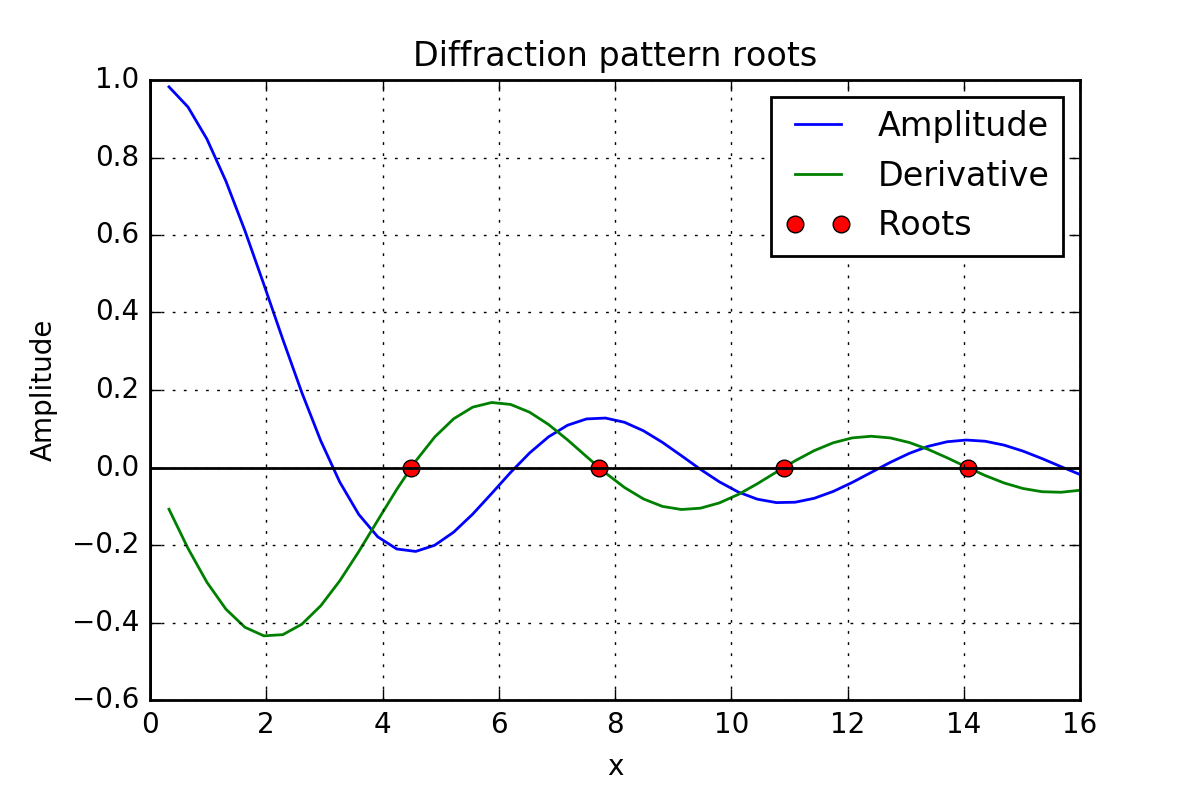
\includegraphics{fraun_root}}
  \end{center}
  \caption{Fraunhoffer diffraction pattern roots}
  \label{fig:fraun_roots}
\end{figure}

\begin{figure}[H]
  \begin{center}
    \scalebox{.8}{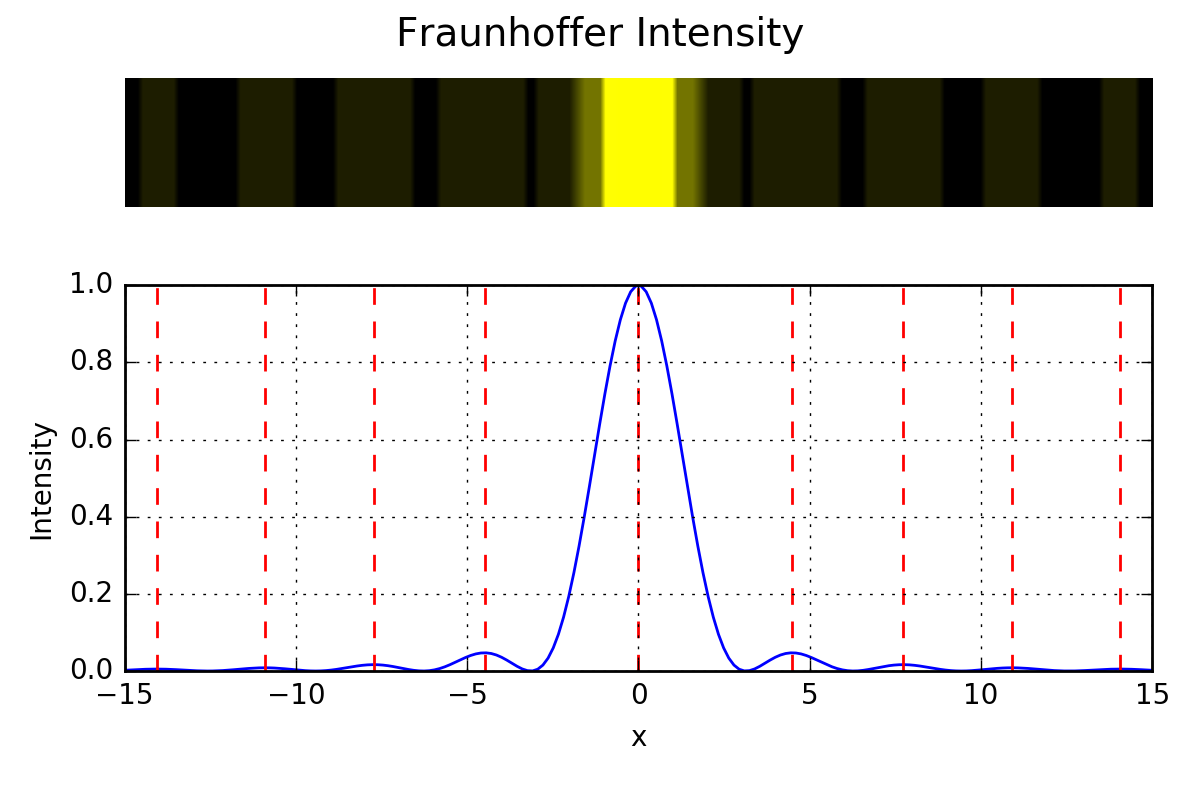
\includegraphics{fraun_int}}
  \end{center}
  \caption{Fraunhoffer intensity and diffraction pattern}
  \label{fig:fraun_int}
\end{figure}


\section{Matrix Computations}

Matrix computations are necessary are prevalent in many physical computations and numerical problems. In this exercise we explore
the GSL library subroutines for matrix computations and property extraction.

For these exercises, the following $3 \times 3$ matrix is used,

\begin{equation}
 \label{eq:mat}
 M = \begin{bmatrix}
       1 & 2 & 3 \\[0.3em]
       2 & 2 & 3 \\[0.3em]
       3 & 3 & 3 \\[0.3em]
      \end{bmatrix}
\end{equation}

The

\begin{equation}
 \label{eq:mat}
 M^{-1} = \begin{bmatrix}
       -1 & 1 & 0 \\[0.3em]
       1 & -2 & 1 \\[0.3em]
       0 & 1 &  -\frac{2}{3}\\[0.3em]
      \end{bmatrix}
\end{equation}

\begin{equation}
 \label{eq:mat}
 \text{det(}M\text{)} = 3.0
\end{equation}

\begin{equation}
 \label{eq:mat}
e_{1} = \begin{bmatrix}
     0.42509 \\[0.3em]
     -0.829153 \\[0.3em]
     0.363048 \\[0.3em]
       \end{bmatrix}\text{,}\quad
e_{2} = \begin{bmatrix}
     0.765677 \\[0.3em]
     0.115485 \\[0.3em]
     -0.632774 \\[0.3em]
       \end{bmatrix}\text{,}\quad
e_{3} = \begin{bmatrix}
     0.482739 \\[0.3em]
     0.546963 \\[0.3em]
     0.683955 \\[0.3em]
       \end{bmatrix}
\end{equation}

\begin{equation}
 \label{eq:mat}
\lambda_{1} = -0.338922 \text{,}\quad
\lambda_{2} = -1.17762 \text{,}\quad
\lambda_{3} = 7.51654
\end{equation}

\begin{figure}[H]
  \begin{center}
    \scalebox{.8}{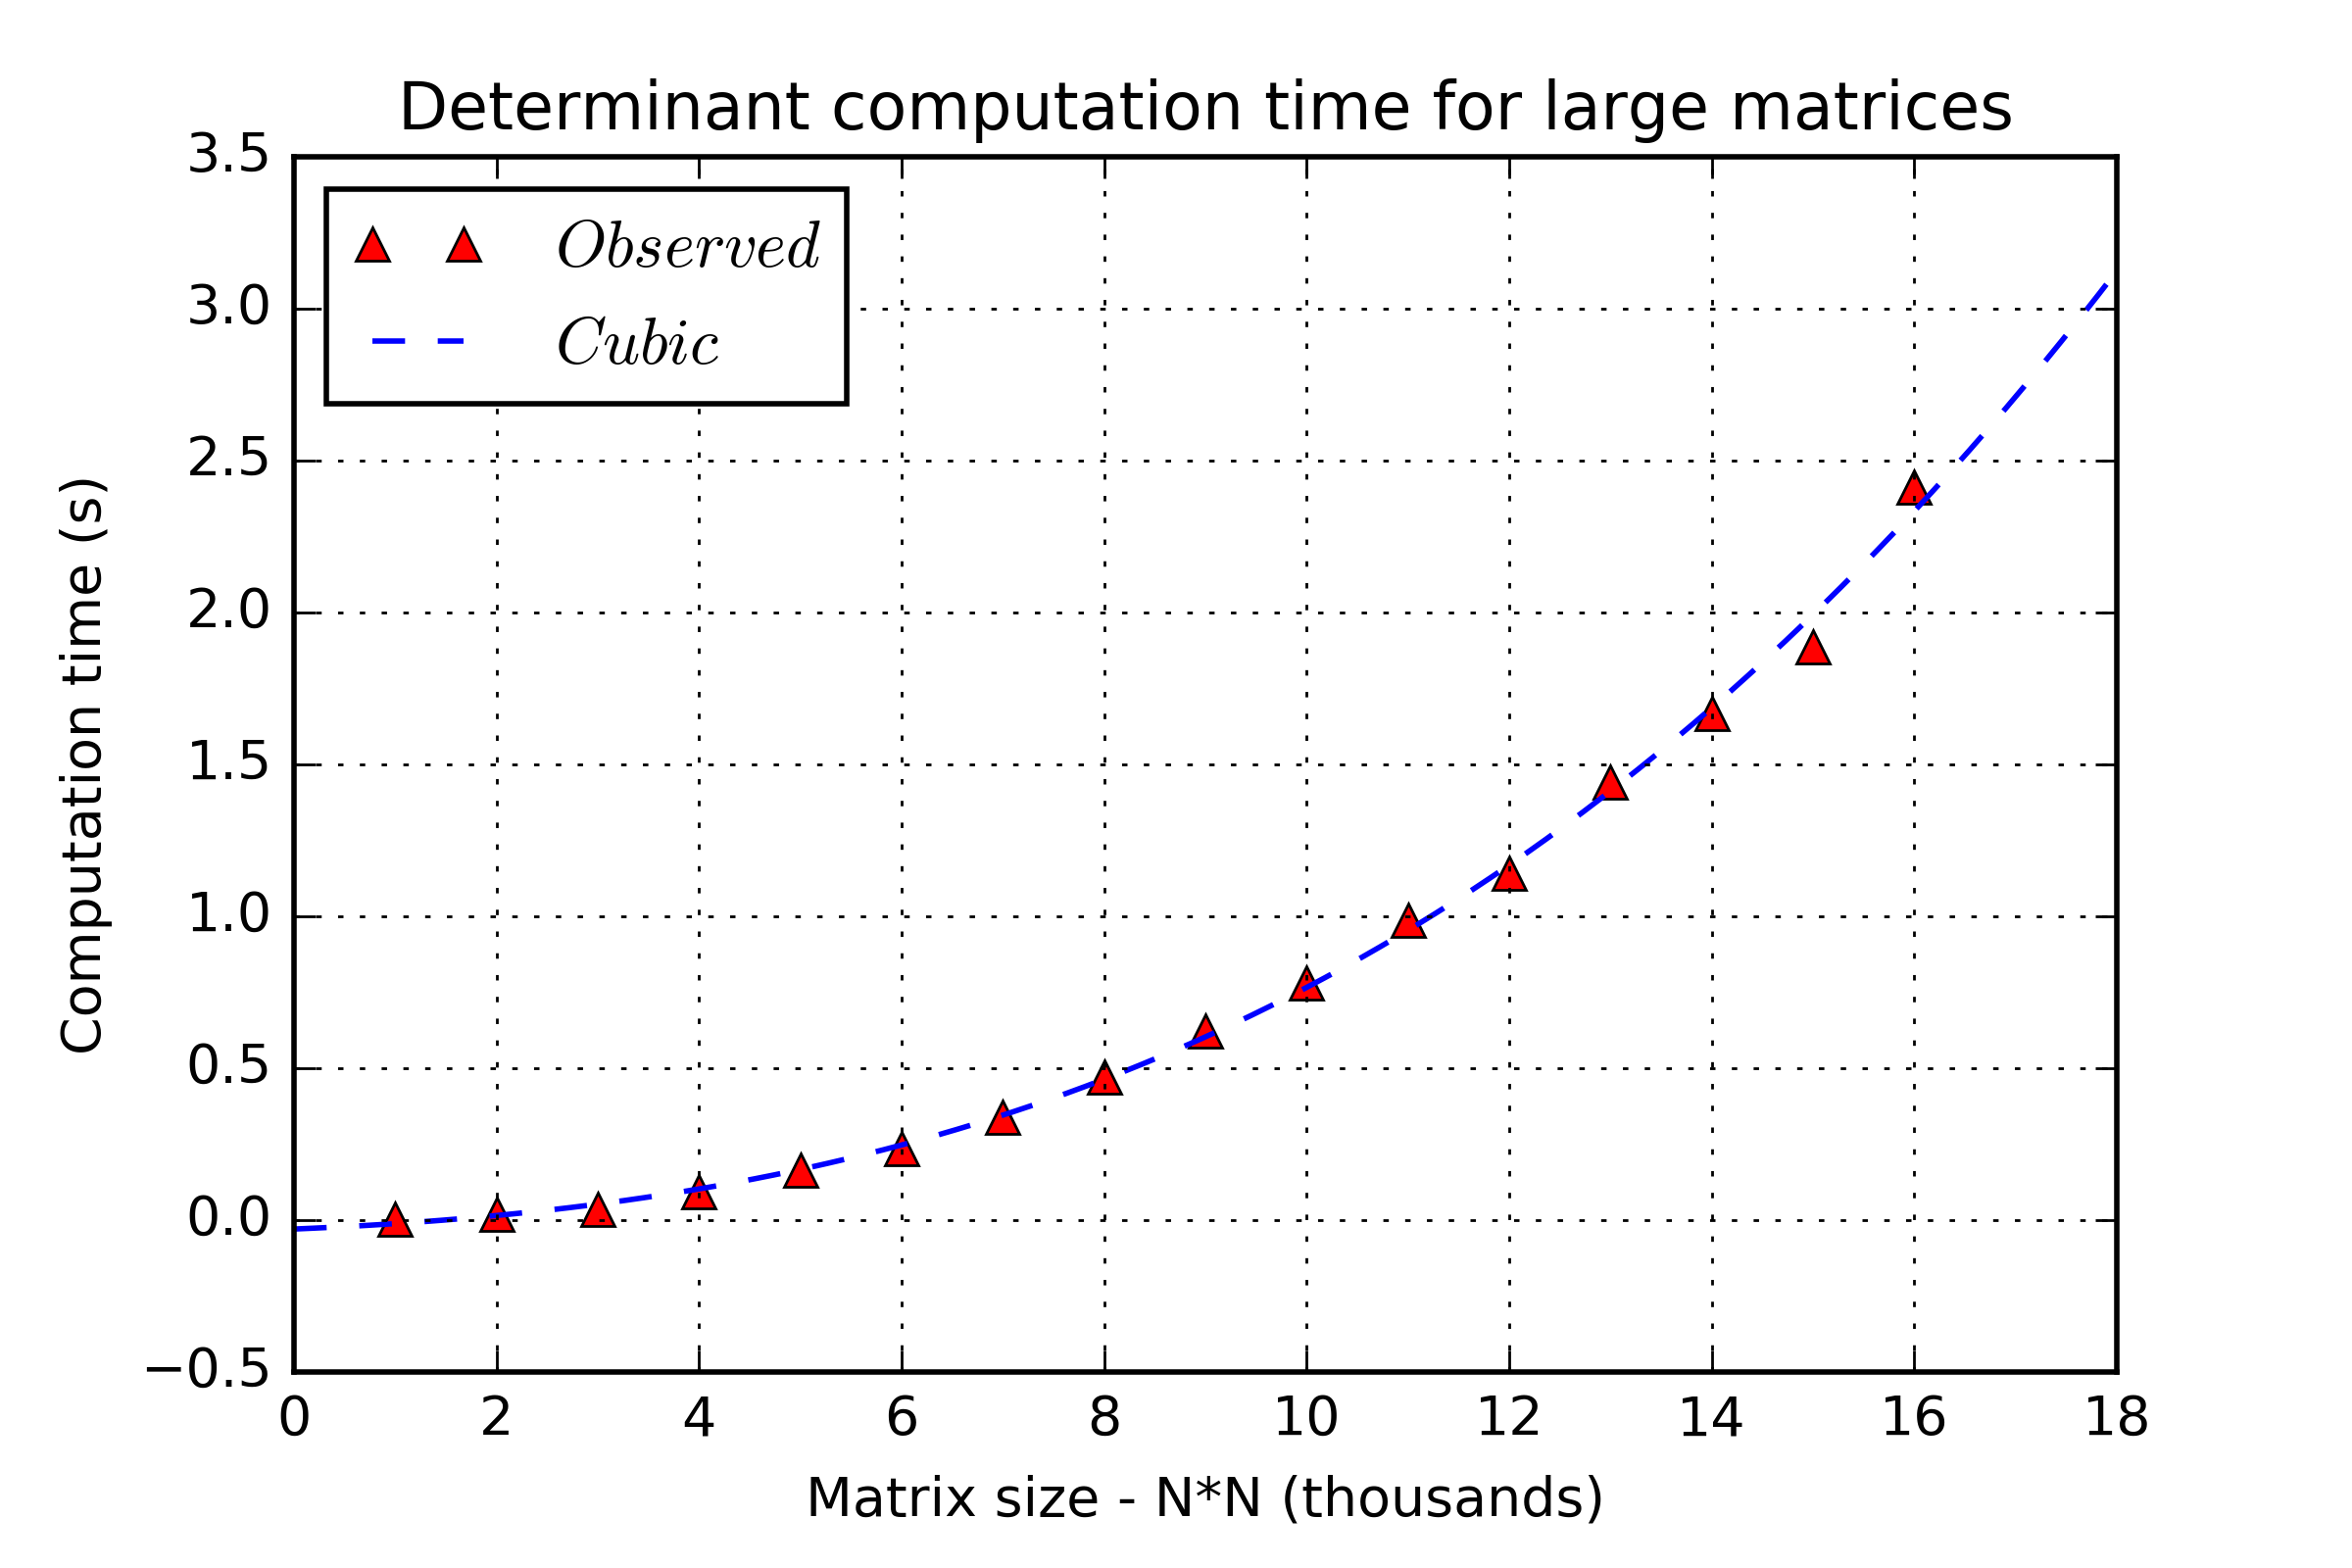
\includegraphics{det_plot}}
  \end{center}
  \caption{Determinant computation time for different matrix sizes}
  \label{fig:mag_susc}
\end{figure}


\section{Method of over-relaxation}

Relax...

\begin{figure}[H]
  \begin{center}
    \scalebox{.8}{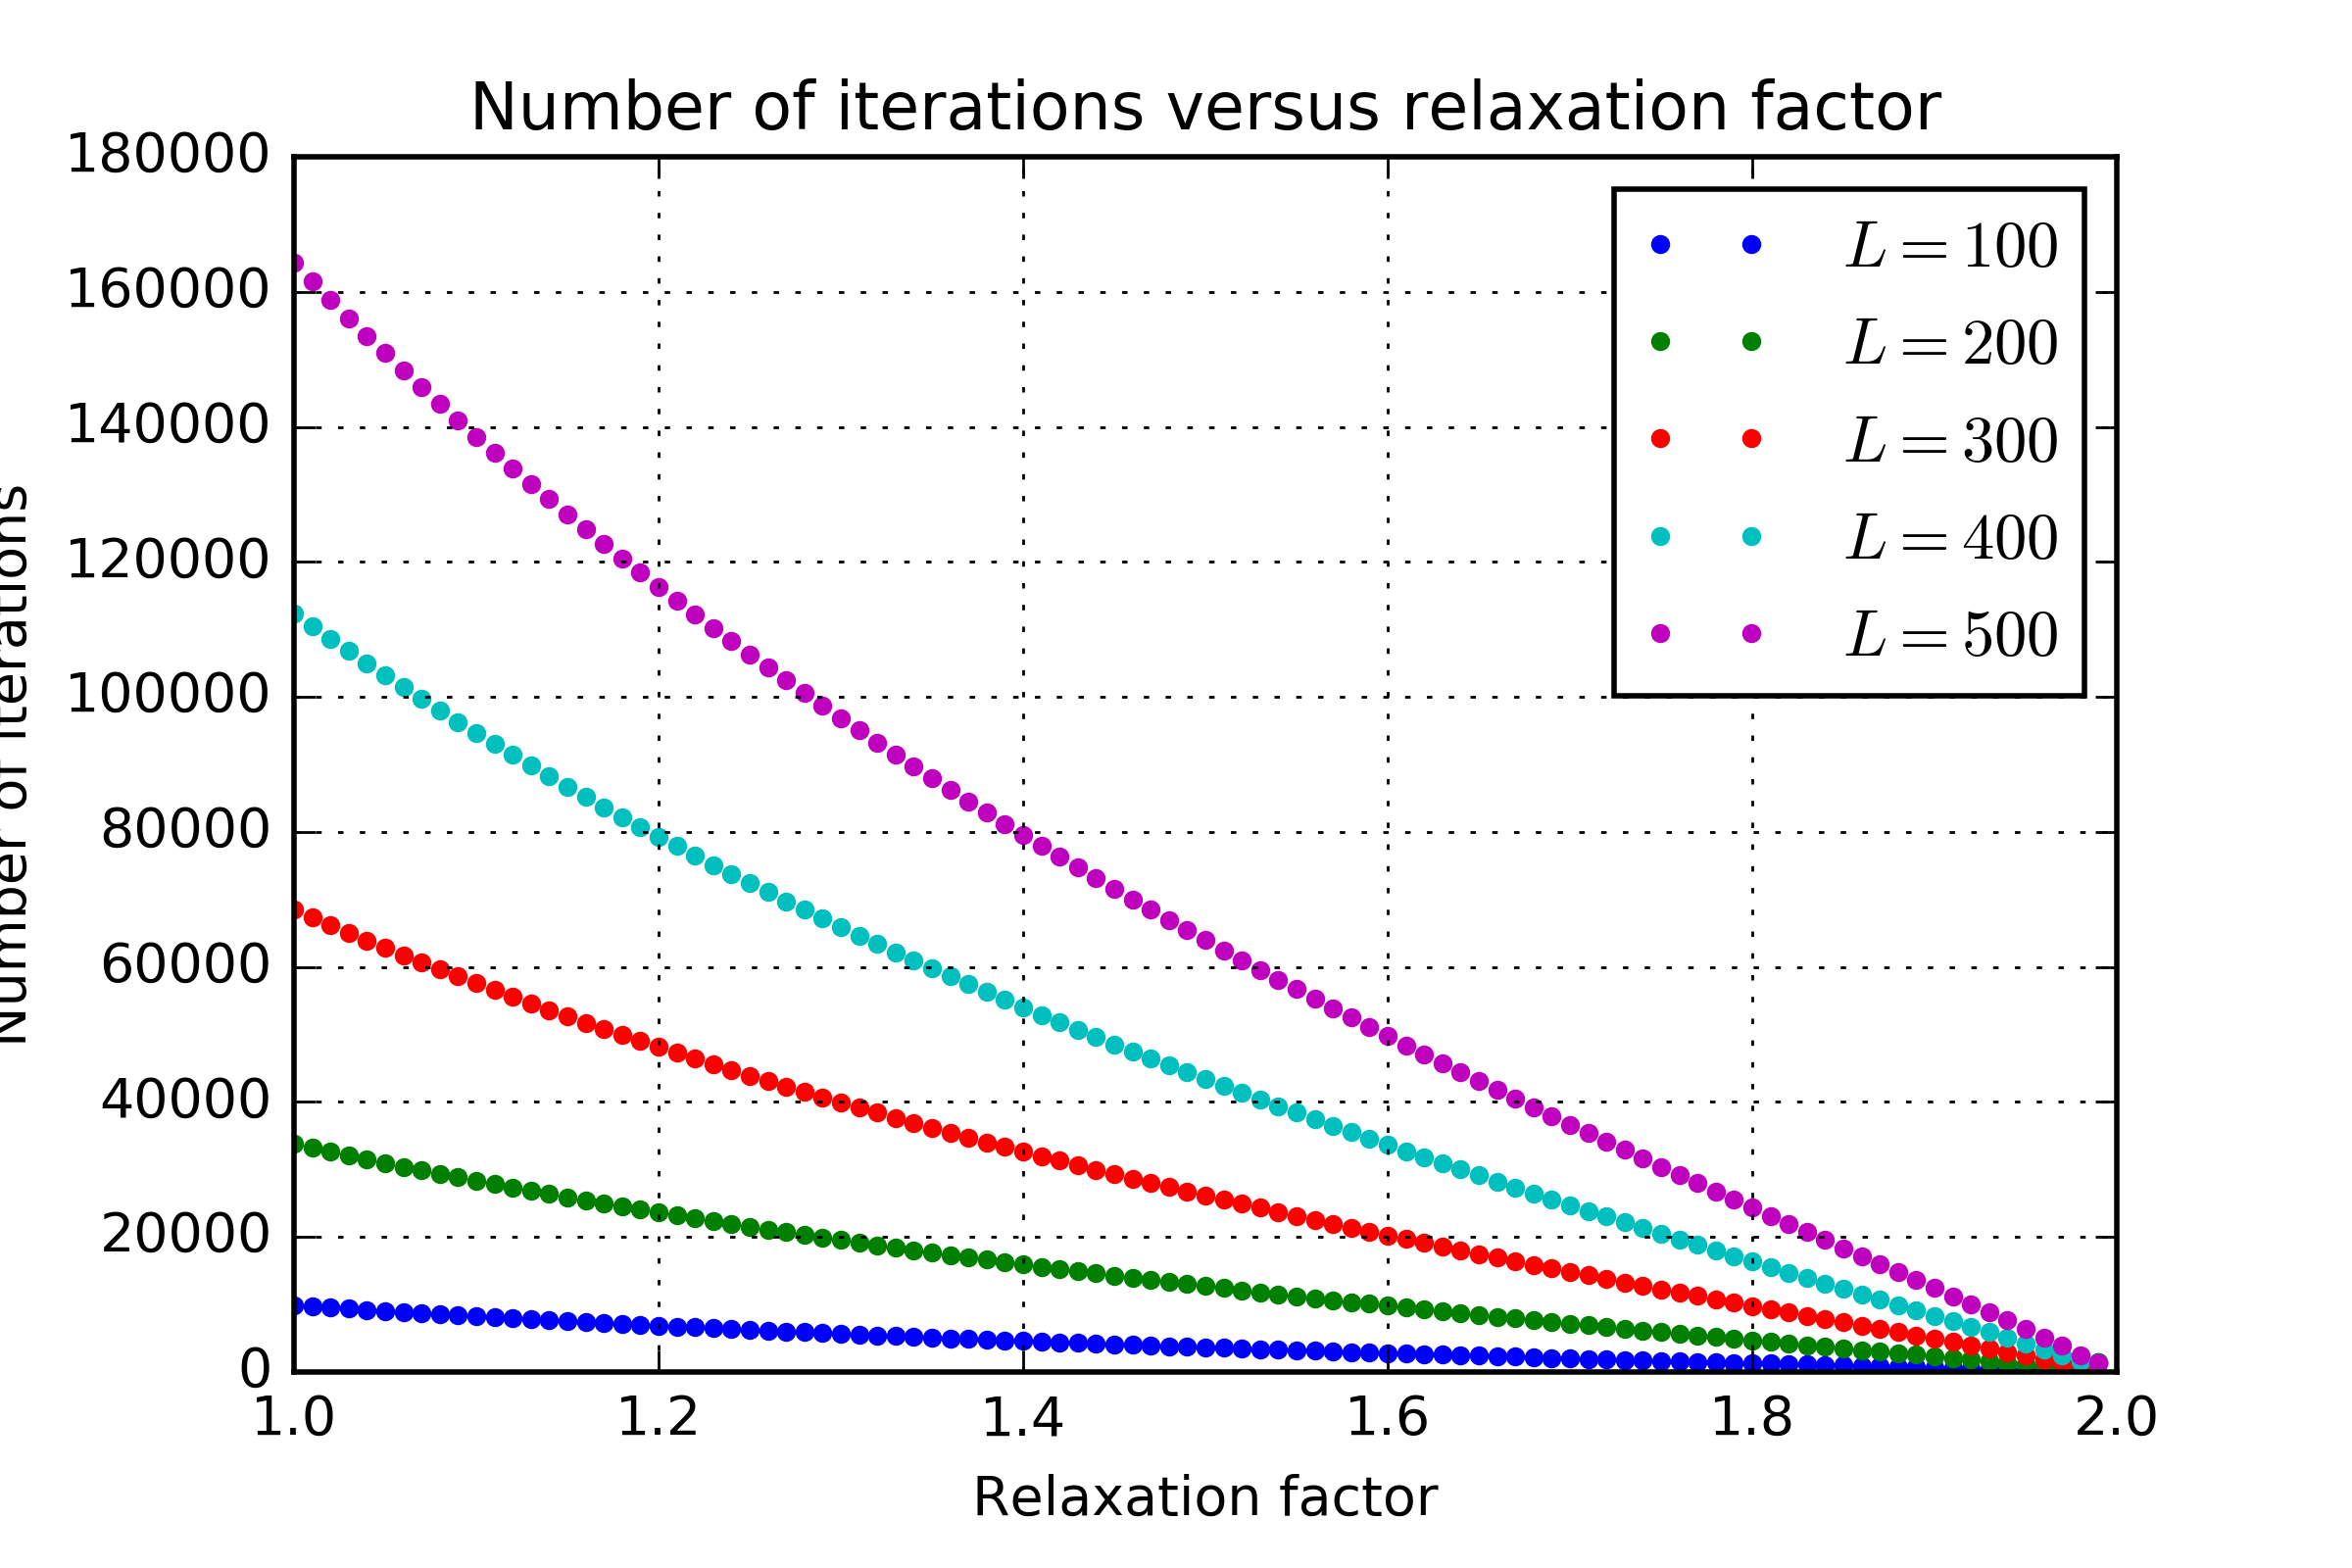
\includegraphics{iter_plot}}
  \end{center}
  \caption{Number of iterations to achieve desired accuracy as a function of the relaxation factor}
  \label{fig:mag_susc}
\end{figure}

\begin{figure}[H]
  \begin{center}
    \scalebox{.8}{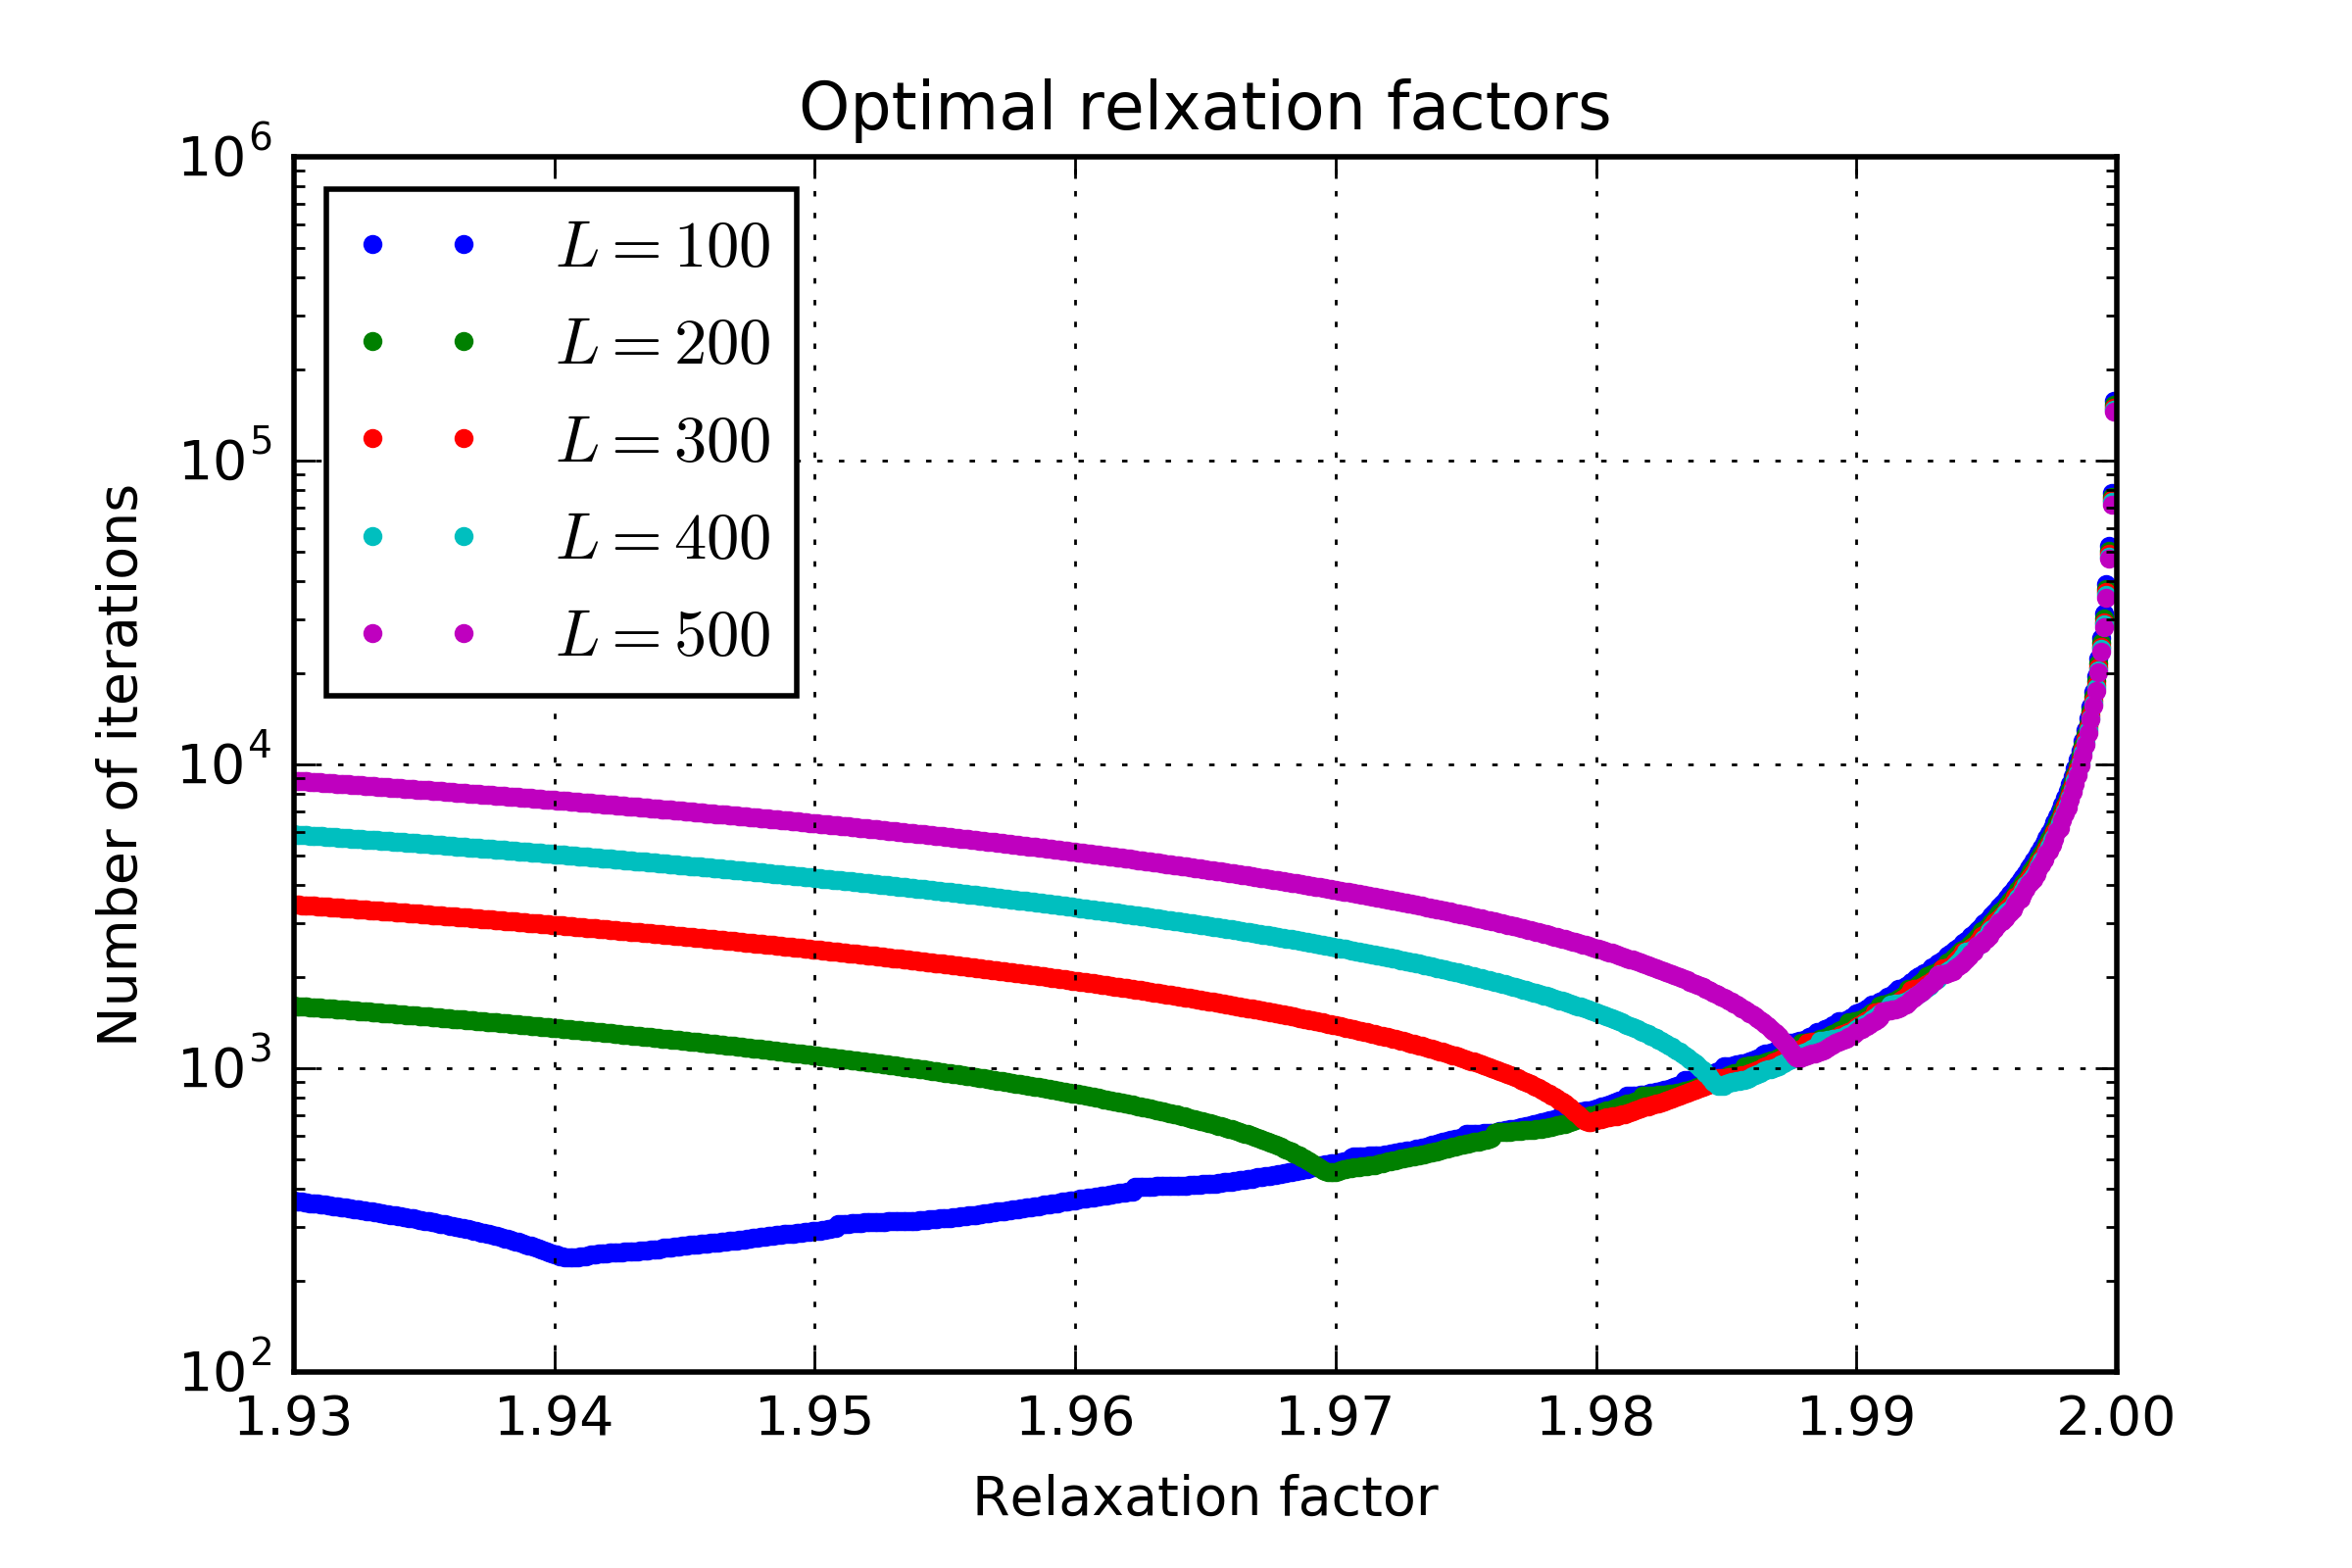
\includegraphics{iter_op_plot}}
  \end{center}
  \caption{Visualization of the optimal relxation factor for different lattice sizes}
  \label{fig:mag_susc}
\end{figure}

\begin{figure}[H]
  \begin{center}
    \scalebox{.8}{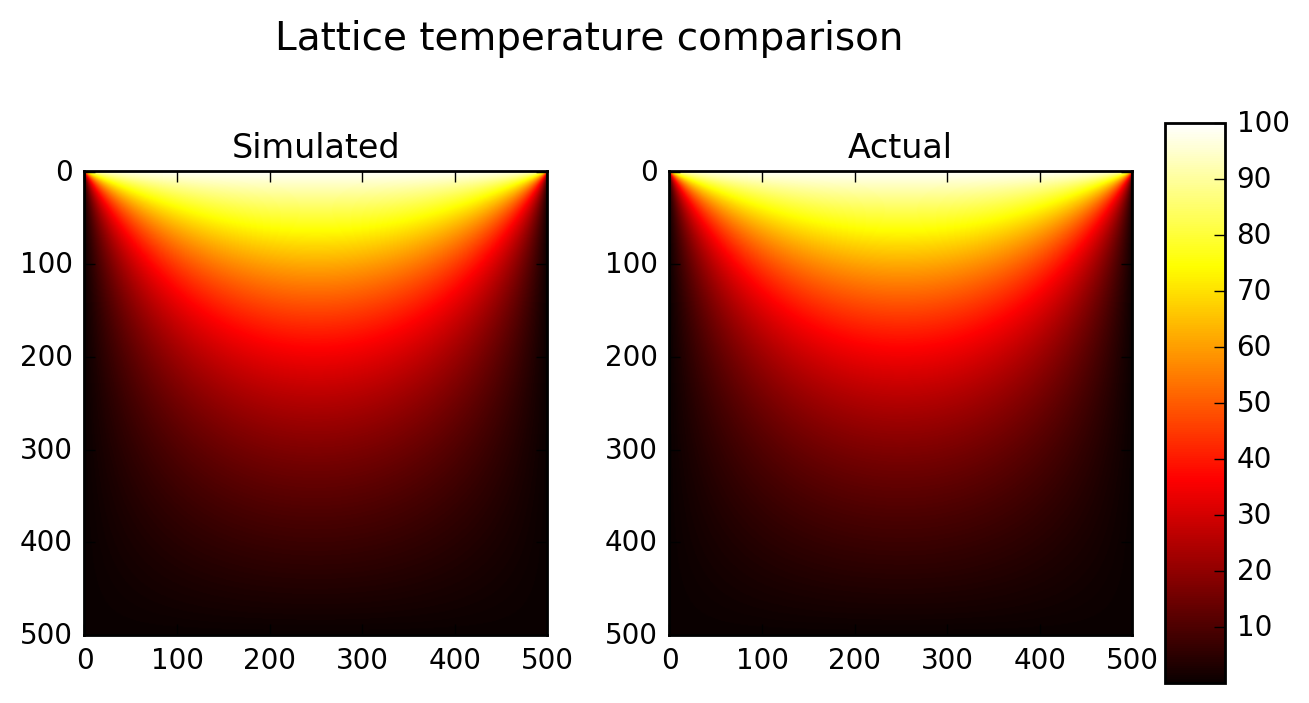
\includegraphics{temp_comp}}
  \end{center}
  \caption{Lattice temperature comparison}
  \label{fig:mag_susc}
\end{figure}

\section{Conclusion}

Conclusion here...

\begin{thebibliography}{9}

  \bibitem{lamport94}
    Wikipedia contributors. \emph{Monte Carlo method.} Wikipedia, The Free Encyclopedia. Wikipedia, The Free Encyclopedia, 28 Mar. 2017.

  \bibitem{lamport94}
    Wikipedia contributors. "Markov chain Monte Carlo." Wikipedia, The Free Encyclopedia. Wikipedia, The Free Encyclopedia, 21 Feb. 2017.

  \bibitem{lamport94}
    Wikipedia contributors. "Square-lattice Ising model." Wikipedia, The Free Encyclopedia. Wikipedia, The Free Encyclopedia, 26 Mar. 2016.

  \bibitem{lamport94}
	  Jacques Kotze,
	  \emph{Introduction to Monte Carlo methods for an Ising model of ferromagnetism}.
    \tt{arXiv:cond-mat.stat-mech/0803.0217}

\end{thebibliography}
\end{document}
